% mnras_template.tex 
%
% LaTeX template for creating an MNRAS paper
%
% v3.0 released 14 May 2015
% (version numbers match those of mnras.cls)
%
% Copyright (C) Royal Astronomical Society 2015
% Authors:
% Keith T. Smith (Royal Astronomical Society)

% Change log
%
% v3.0 May 2015
%    Renamed to match the new package name
%    Version number matches mnras.cls
%    A few minor tweaks to wording
% v1.0 September 2013
%    Beta testing only - never publicly released
%    First version: a simple (ish) template for creating an MNRAS paper

%%%%%%%%%%%%%%%%%%%%%%%%%%%%%%%%%%%%%%%%%%%%%%%%%%
% Basic setup. Most papers should leave these options alone.
\documentclass[fleqn,usenatbib]{mnras}

% MNRAS is set in Times font. If you don't have this installed (most LaTeX
% installations will be fine) or prefer the old Computer Modern fonts, comment
% out the following line
\usepackage{newtxtext,newtxmath}
% Depending on your LaTeX fonts installation, you might get better results with one of these:
%\usepackage{mathptmx}
%\usepackage{txfonts}

% Use vector fonts, so it zooms properly in on-screen viewing software
% Don't change these lines unless you know what you are doing
\usepackage[T1]{fontenc}

% Allow "Thomas van Noord" and "Simon de Laguarde" and alike to be sorted by "N" and "L" etc. in the bibliography.
% Write the name in the bibliography as "\VAN{Noord}{Van}{van} Noord, Thomas"
\DeclareRobustCommand{\VAN}[3]{#2}
\let\VANthebibliography\thebibliography
\def\thebibliography{\DeclareRobustCommand{\VAN}[3]{##3}\VANthebibliography}


%%%%% AUTHORS - PLACE YOUR OWN PACKAGES HERE %%%%%

% Only include extra packages if you really need them. Common packages are:
\usepackage{graphicx}	% Including figure files
\usepackage{amsmath}	% Advanced maths commands
% \usepackage{amssymb}	% Extra maths symbols

\usepackage[dvipsnames]{xcolor}

%%%%%%%%%%%%%%%%%%%%%%%%%%%%%%%%%%%%%%%%%%%%%%%%%%

%%%%% AUTHORS - PLACE YOUR OWN COMMANDS HERE %%%%%

% Please keep new commands to a minimum, and use \newcommand not \def to avoid
% overwriting existing commands. Example:
%\newcommand{\pcm}{\,cm$^{-2}$}	% per cm-squared

\newcommand{\zach}[1]{\textcolor{BurntOrange}{\textbf{Zach: #1}}}

%%%%%%%%%%%%%%%%%%%%%%%%%%%%%%%%%%%%%%%%%%%%%%%%%%

%%%%%%%%%%%%%%%%%%% TITLE PAGE %%%%%%%%%%%%%%%%%%%

% Title of the paper, and the short title which is used in the headers.
% Keep the title short and informative.
\title[Halo21 CGM Modeling Challenge]{The Halo21 Absorption Modeling Challenge: [Takeaway Title Message Here]}

% The list of authors, and the short list which is used in the headers.
% If you need two or more lines of authors, add an extra line using \newauthor
\author[]{
The Halo 21 Absorption Modeling Group
\\
% List of institutions
$^{1}$TBD\\
}

% These dates will be filled out by the publisher
\date{Accepted XXX. Received YYY; in original form ZZZ}

% Enter the current year, for the copyright statements etc.
\pubyear{2015}

% Don't change these lines
\begin{document}
\label{firstpage}
\pagerange{\pageref{firstpage}--\pageref{lastpage}}
\maketitle

% Abstract of the paper
\begin{abstract}
This is a simple template for authors to write new MNRAS papers.
The abstract should briefly describe the aims, methods, and main results of the paper.
It should be a single paragraph not more than 250 words (200 words for Letters).
No references should appear in the abstract.
\end{abstract}

% Select between one and six entries from the list of approved keywords.
% Don't make up new ones.
\begin{keywords}
keyword1 -- keyword2 -- keyword3
\end{keywords}

%%%%%%%%%%%%%%%%%%%%%%%%%%%%%%%%%%%%%%%%%%%%%%%%%%

%%%%%%%%%%%%%%%%% BODY OF PAPER %%%%%%%%%%%%%%%%%%
\section{NOTES FOR AUTHORS}

\subsection{KEY FOR COAUTHORS}

\textbf{Bold: Notes for things to implement.}
\textit{Italics: Rough text, needs polishing.}
Normal: Normal text, polished enough to be included in a draft.

\subsection{Outstanding Questions/Discussion Points}

% Who is the target audience?
\textbf{Who is the target audience?}
Imagine sitting down with the target audience.
What are the most important points we want to convey?
In particular, what could they really use?

\section{Introduction}


\section{Data samples}

\subsection{Highly idealized}

\textbf{This corresponds to sample0.}

\zach{Cameron, would you be able to write down the steps you took?}

\subsection{Informed by cosmological simulations}

\textbf{This corresponds to sample1.}

\zach{Nastasha, would you be able to write down the steps you took?}

\subsection{Drawn from high resolution simulations}

\textbf{This corresponds to sample2.}

\zach{Nir, would you be able to write down the steps you took?}

% C IV and changed redshift
\textit{
We changed the redshift to $z=0.13$ to bring \ion{C}{IV} into the observable range for the COS gratings.
Note that the simulations were run at $z=2$, including a $z=2$ UVB background.
However, the ionization fractions were calculated in post-processing via Trident using a $z=0.13$ UVB background.
}

\section{Observational Modeling}

\section{Results}

\subsection{Highly idealized}

\begin{figure*}
    \centering
    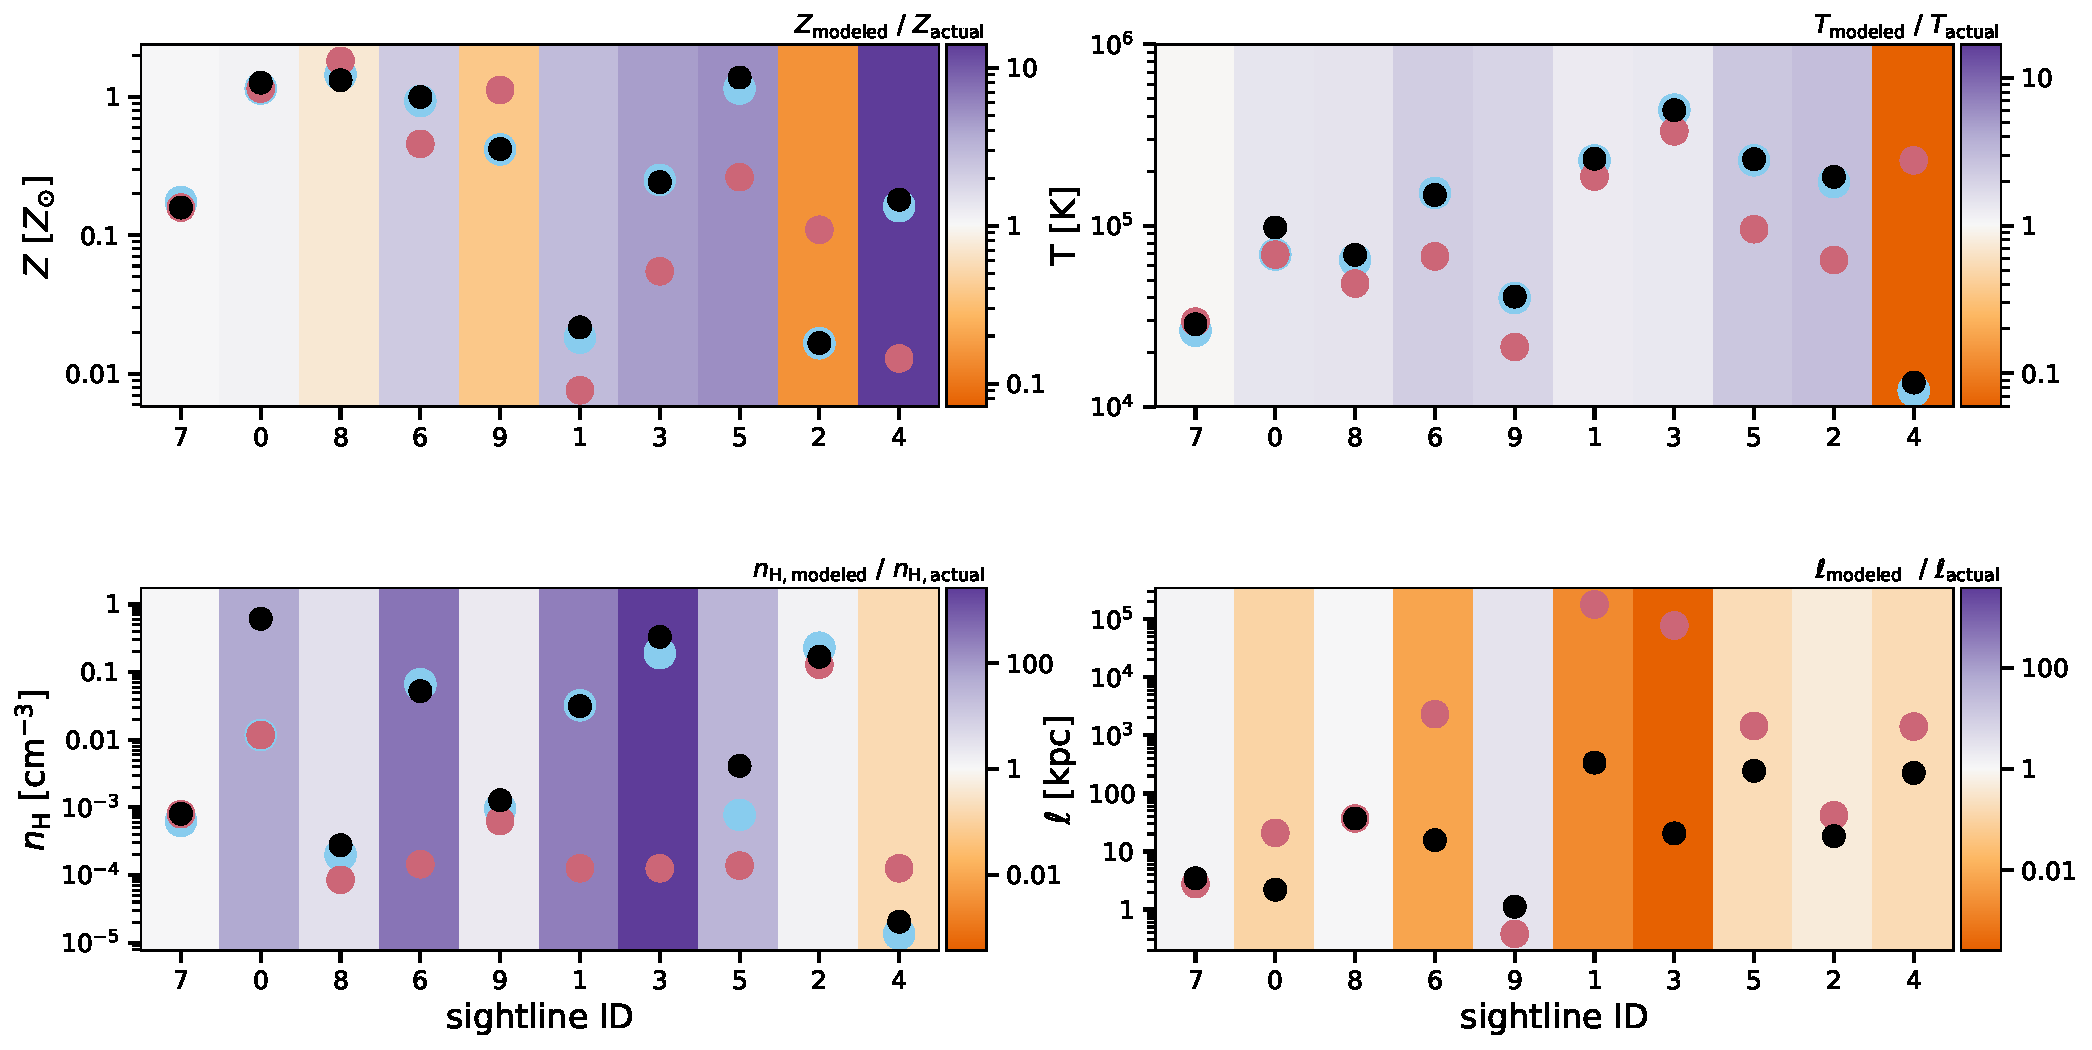
\includegraphics[width=\textwidth]{figures/sample0/comparison.pdf}
    \caption{
    Comparison in highly idealized scenario.
    }
    \label{f: idealized}
\end{figure*}

\begin{figure}
    \centering
    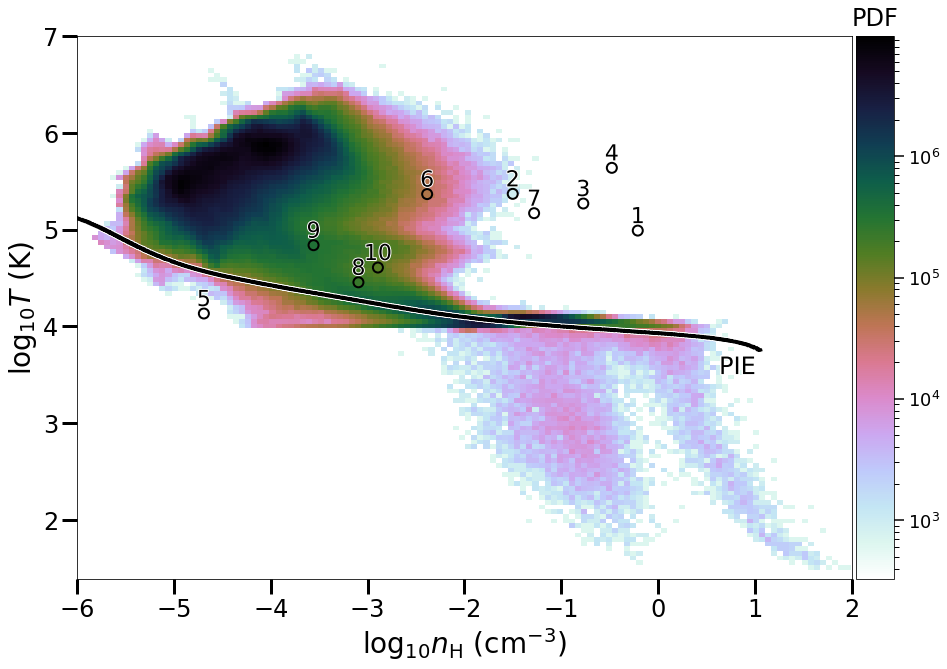
\includegraphics[width=\columnwidth]{figures/sample0/phase_space.png}
    \caption{
    \textbf{Set colorbar by percent enclosed.}
    \textbf{Use consistent axes: all log, or no log.}
    }
    \label{f: idealized explanation}
\end{figure}

\begin{figure*}
    \centering
    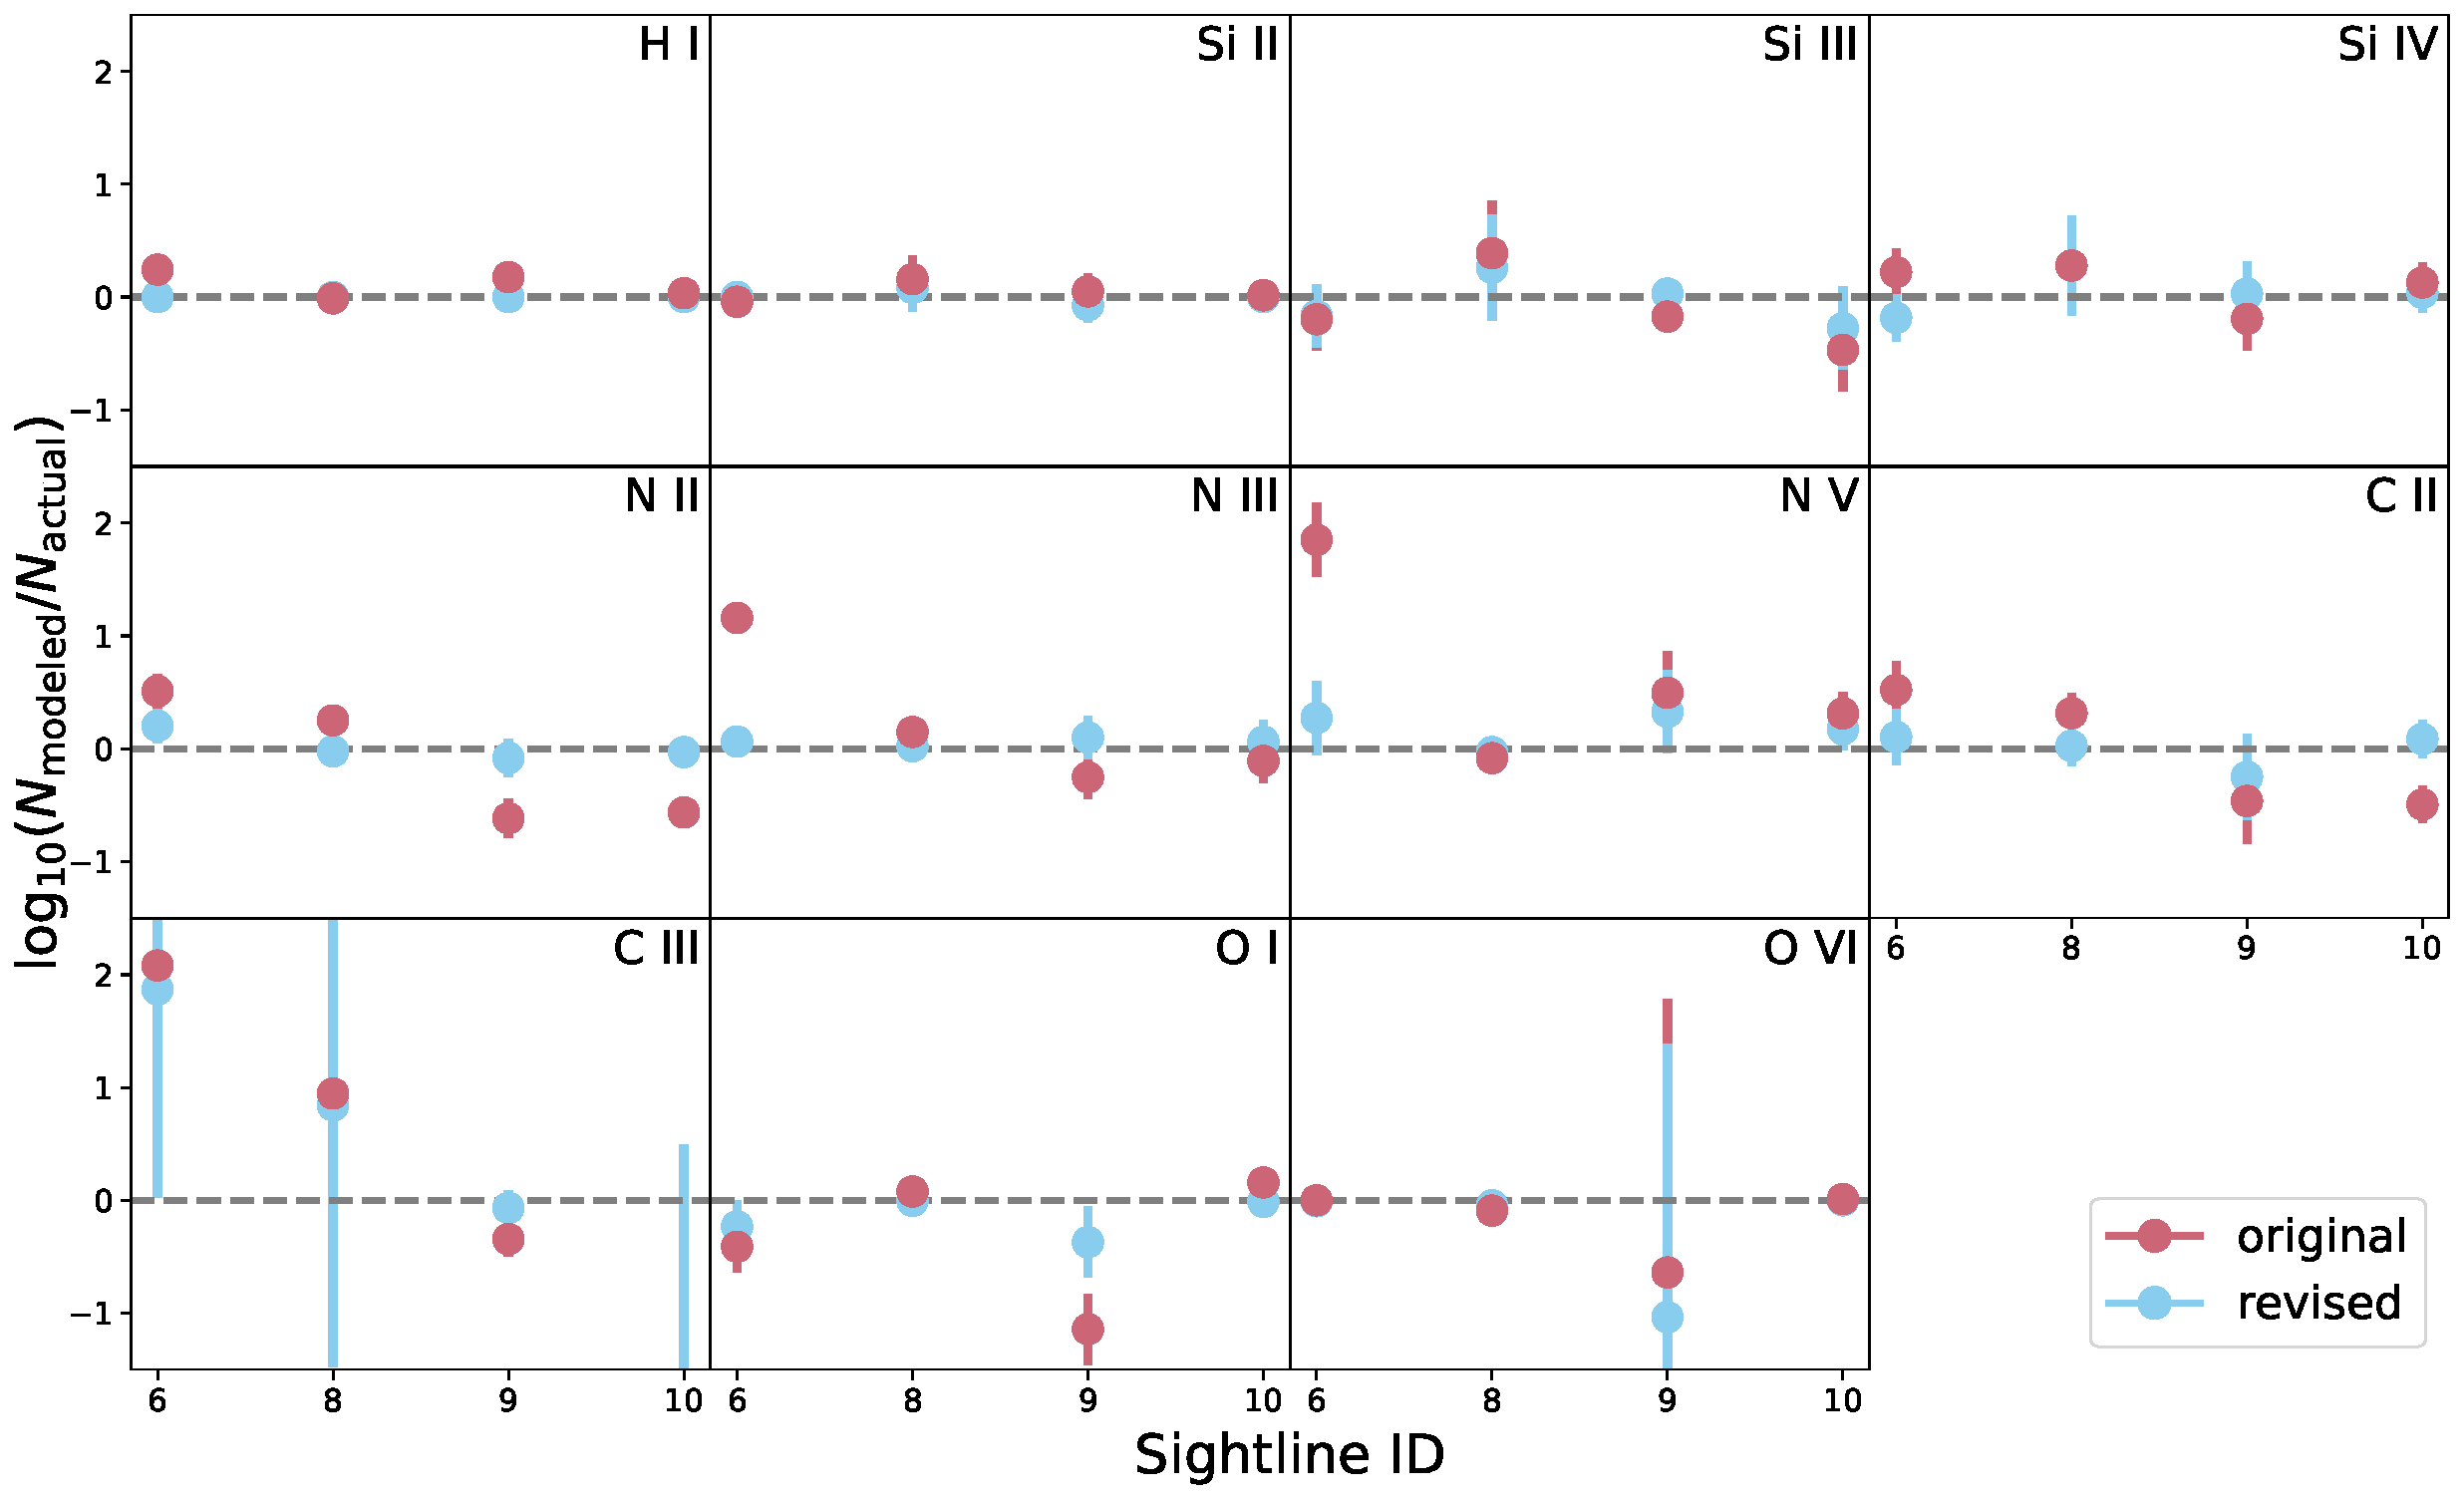
\includegraphics[width=\textwidth]{figures/sample0/column_den.pdf}
    \label{f: column density agreement}
\end{figure*}

\subsection{Informed by cosmological simulations}

\begin{figure}
    \centering
    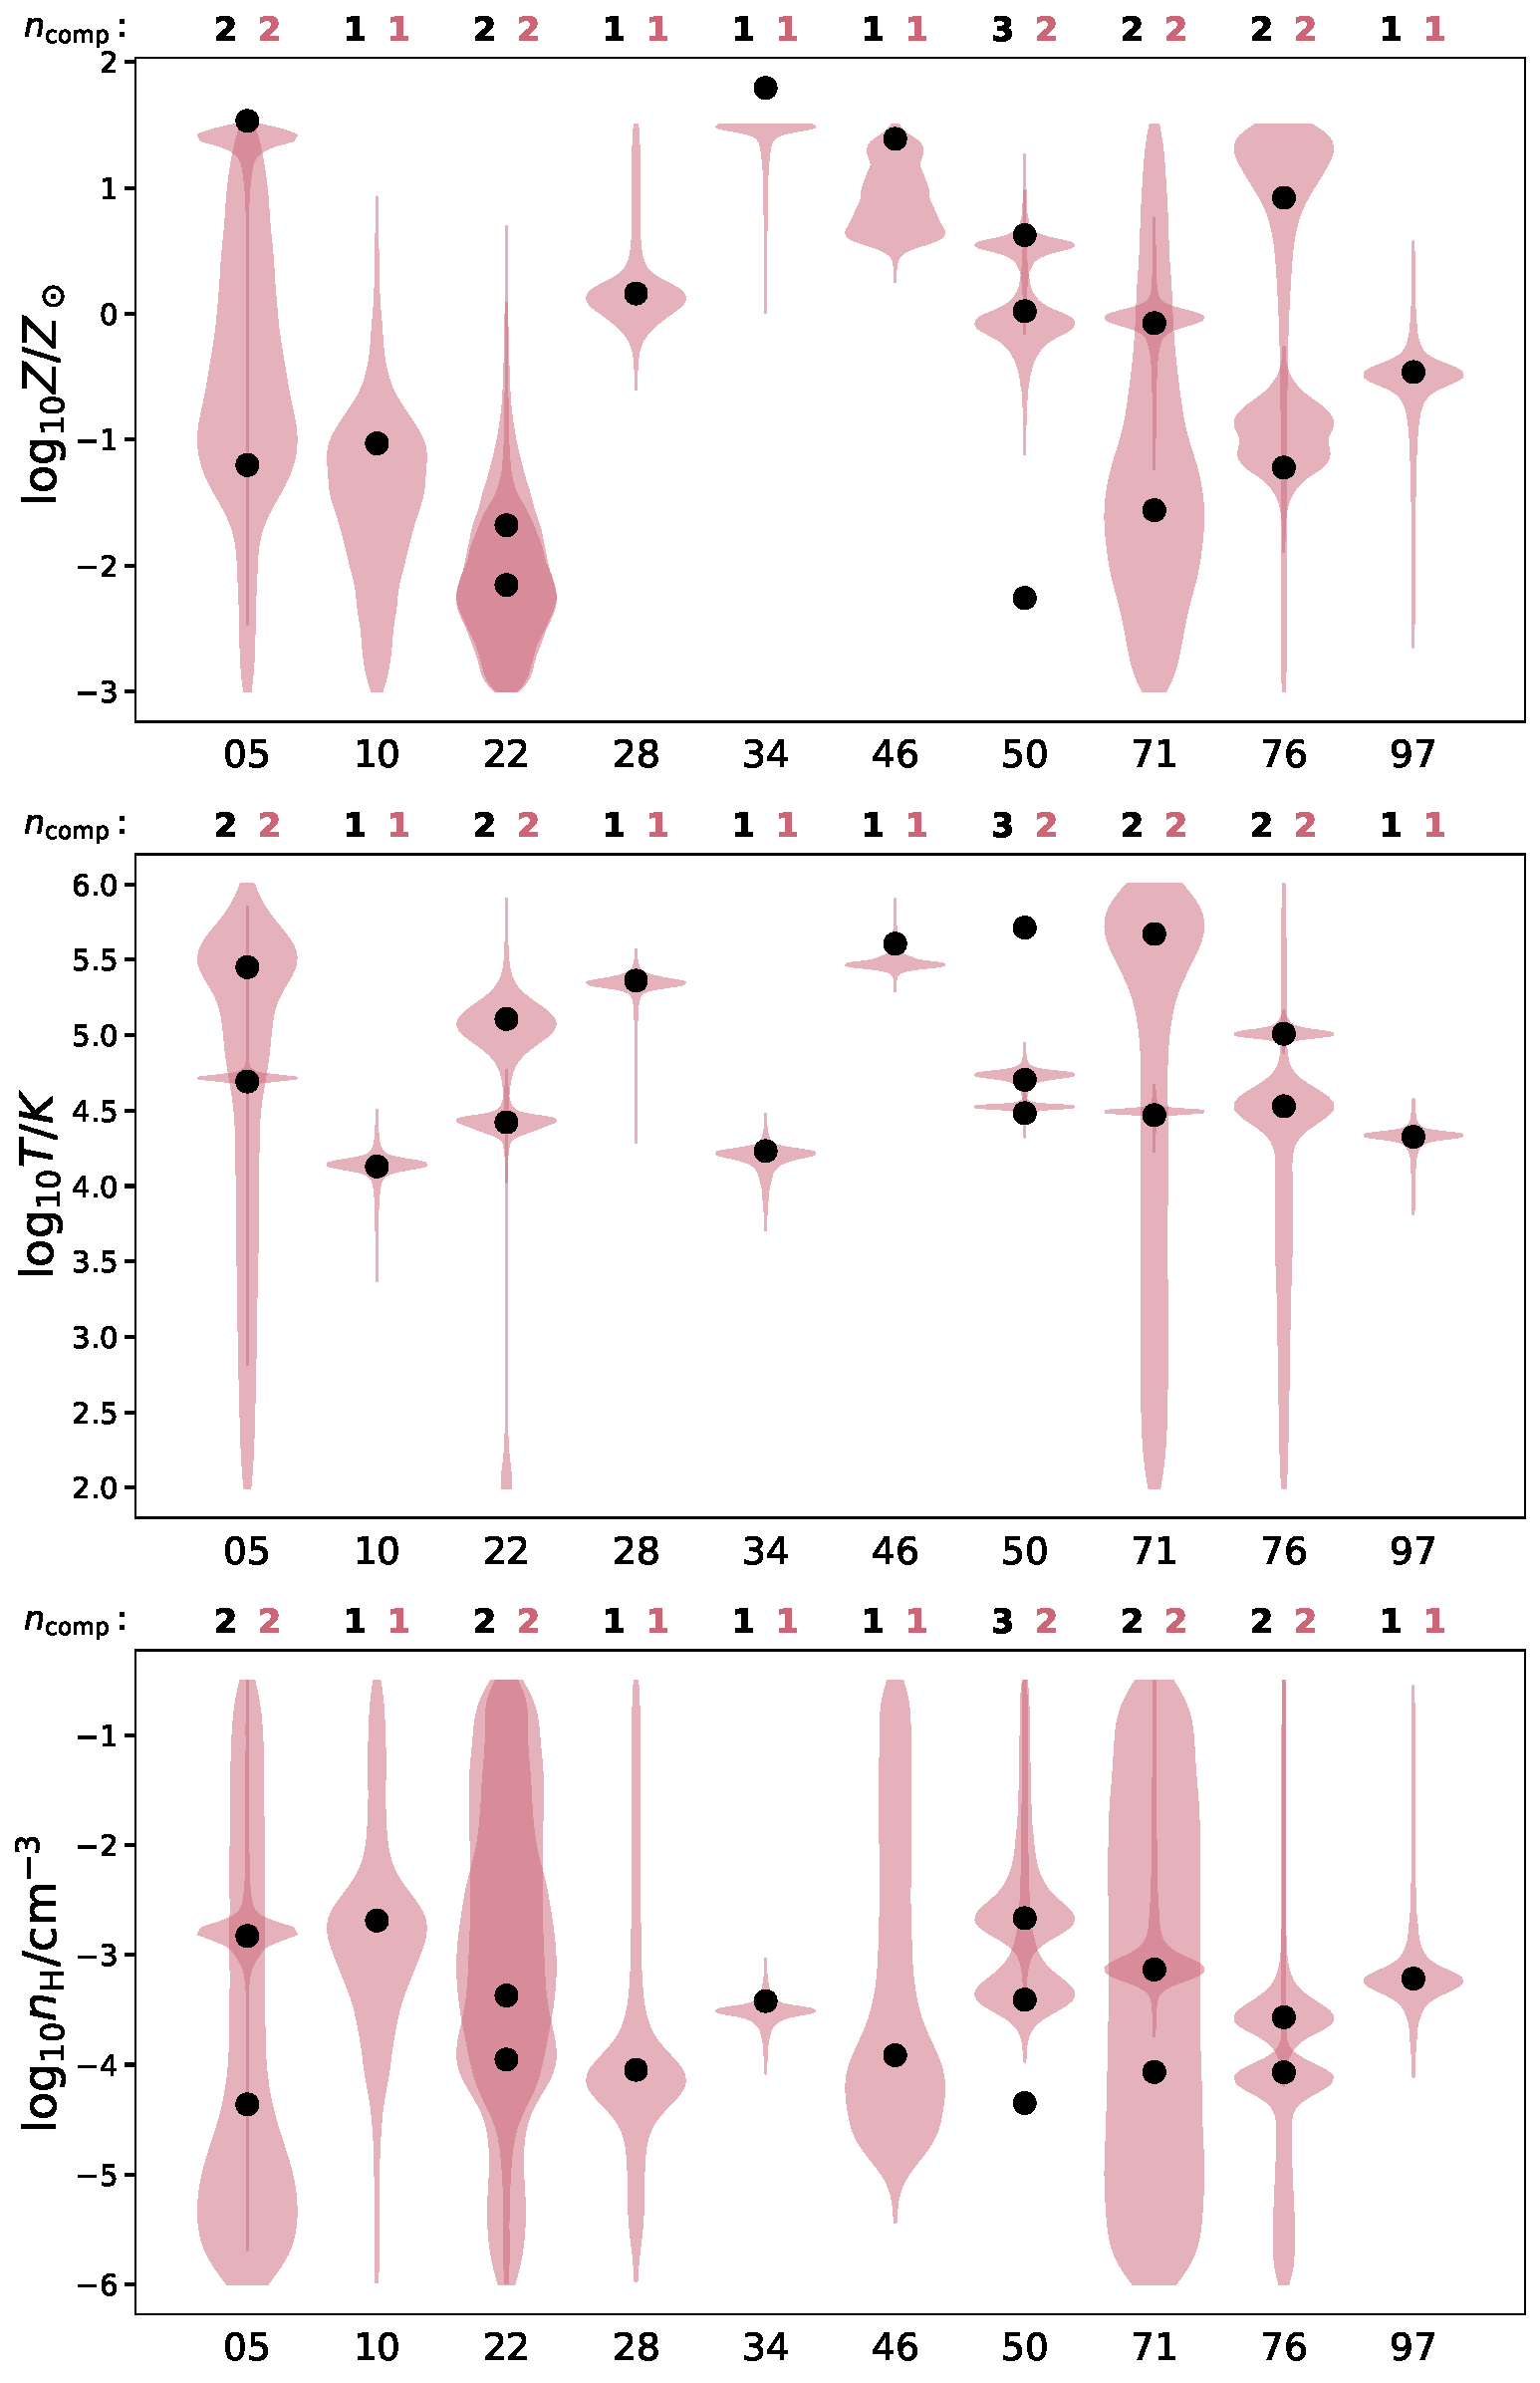
\includegraphics[width=\columnwidth]{figures/sample1/comparison.pdf}
    \caption{
    Comparison informed by cosmological simulations.
    }
    \label{f: informed}
\end{figure}

\subsection{Drawn from high resolution simulations}

\begin{figure*}
    \centering
    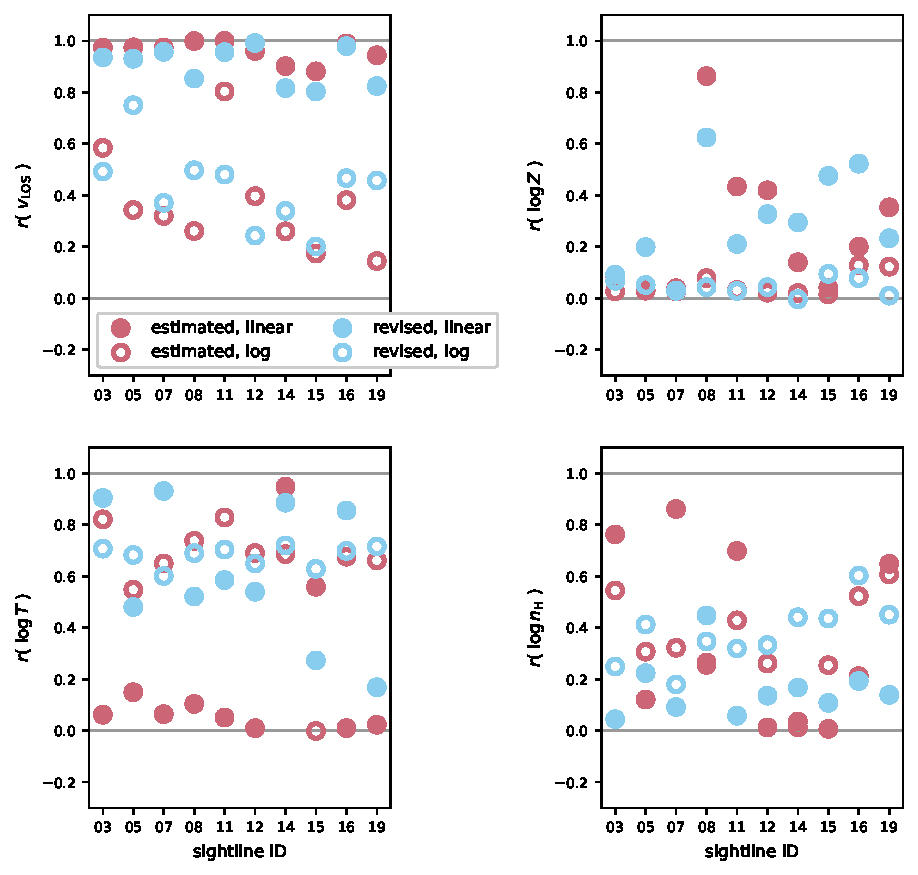
\includegraphics[width=\textwidth]{figures/sample2/correlations.pdf}
    \label{f: column density agreement}
\end{figure*}

\section{Conclusions}

The last numbered section should briefly summarise what has been done, and describe
the final conclusions which the authors draw from their work.

\section*{Acknowledgements}

The Acknowledgements section is not numbered. Here you can thank helpful
colleagues, acknowledge funding agencies, telescopes and facilities used etc.
Try to keep it short.

%%%%%%%%%%%%%%%%%%%%%%%%%%%%%%%%%%%%%%%%%%%%%%%%%%
\section*{Data Availability}

 
The inclusion of a Data Availability Statement is a requirement for articles published in MNRAS. Data Availability Statements provide a standardised format for readers to understand the availability of data underlying the research results described in the article. The statement may refer to original data generated in the course of the study or to third-party data analysed in the article. The statement should describe and provide means of access, where possible, by linking to the data or providing the required accession numbers for the relevant databases or DOIs.




%%%%%%%%%%%%%%%%%%%% REFERENCES %%%%%%%%%%%%%%%%%%

% The best way to enter references is to use BibTeX:

\bibliographystyle{mnras}
\bibliography{example} % if your bibtex file is called example.bib


% Alternatively you could enter them by hand, like this:
% This method is tedious and prone to error if you have lots of references
%\begin{thebibliography}{99}
%\bibitem[\protect\citeauthoryear{Author}{2012}]{Author2012}
%Author A.~N., 2013, Journal of Improbable Astronomy, 1, 1
%\bibitem[\protect\citeauthoryear{Others}{2013}]{Others2013}
%Others S., 2012, Journal of Interesting Stuff, 17, 198
%\end{thebibliography}

%%%%%%%%%%%%%%%%%%%%%%%%%%%%%%%%%%%%%%%%%%%%%%%%%%

%%%%%%%%%%%%%%%%% APPENDICES %%%%%%%%%%%%%%%%%%%%%

\appendix

\section{Some extra material}

If you want to present additional material which would interrupt the flow of the main paper,
it can be placed in an Appendix which appears after the list of references.

%%%%%%%%%%%%%%%%%%%%%%%%%%%%%%%%%%%%%%%%%%%%%%%%%%


% Don't change these lines
\bsp	% typesetting comment
\label{lastpage}
\end{document}

% End of mnras_template.tex
